\documentclass[../../main.tex]{subfiles}


\begin{document}

\subsection*{(a)}
There are 4982 Applications with an average throughput time of 21.904 as determined using the following Process:\\
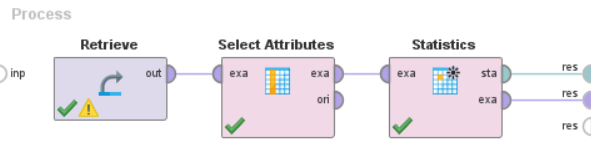
\includegraphics[width=\textwidth]{img/QUESTION_5a_PROCESS_average_throughput_time.png}

Using Celonis Process AI on our Dataset we learn that the most frequent variant (happy path) happens 320 times. This variant can be seen below.\\
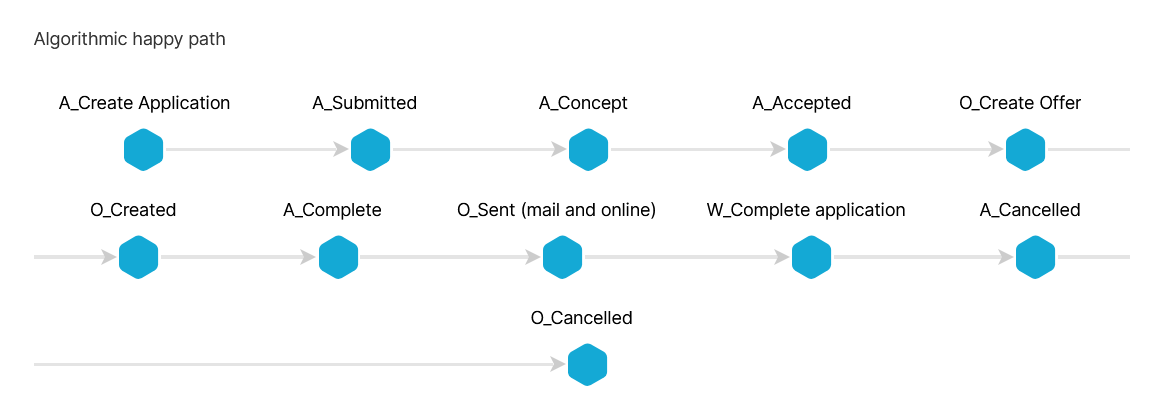
\includegraphics[width=\textwidth]{img/QUESTION_5a_happy_path.png}

The following graph shows the frequency distribution of the throughput times. As one can see they are initially quite high and eventually deteriorate in frequency until the 29-33 Day, where they spike again and after that deteriorate quickly again. The reason for the spike at 29-33 Days is probably that a new month begins/ends at this time. Therefore many applications will likely be terminated at this time for administrative reasons.\\
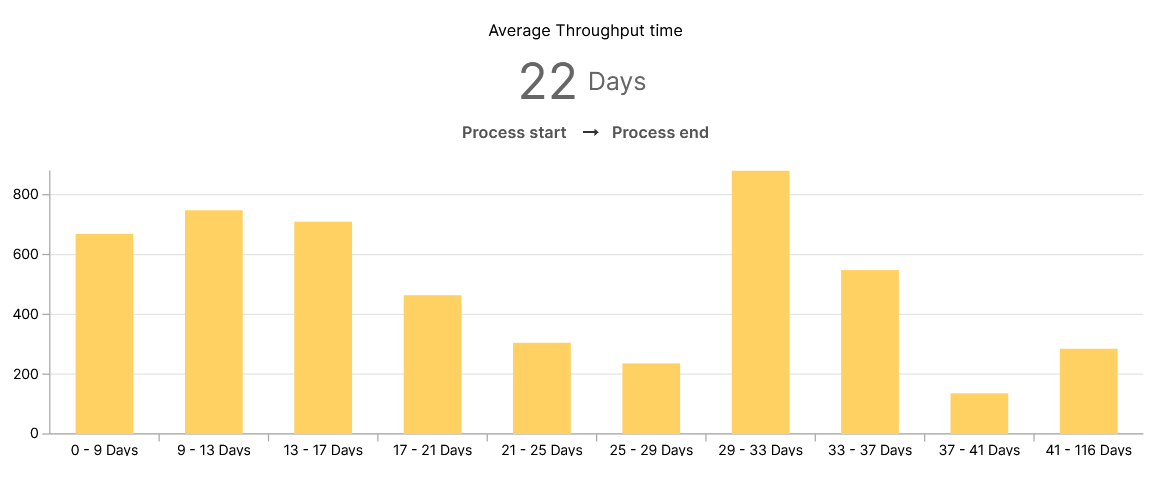
\includegraphics[width=\textwidth]{img/QUESTION_5a_throughput_time_distribution.png}





\subsection*{(b)}
\subsection*{(c)}
\subsection*{(d)}



\end{document}